\section{Summary}
Hebbian learning is a neuroscientific theory to explain synaptic plasticity - the ability of the brain to adapt neurons to learn new tasks. It is characterised by the following two mechanisms. Firstly, a synapse connecting two neurons that are repeatedly active at the same time becomes increasingly strong resulting in an interassociation between the cells. Secondly, the theory suggests a mechanism that causes different synapses to compete with each other such that the strengthening of one synapse leads to the weakening of another. 
This paper now explores an explanation for synaptic plasticity that does not require unrealistic global intracellular signaling, preset activity or synaptic efficacy levels. Instead, Song et. al argue that the timing of pre- and postsynaptic activity alone leads to competitive Hebbian learning. The main finding is that STDP leads to a stationary distribution of synaptic conductances that results in a balanced, irregulary firing regime of the postsynaptic neuron. This enables competition among the inputs to get control over the postsynaptic spike timing.
\newline\newline
The foundation for the exploration of STDP is given by the function $F$ that has been experimentally observed to describe the dependence of synaptic modification on spike timing:

\begin{minipage}{0.5\textwidth}
	$$F(\Delta t ) = \begin{cases}
	A_+ \exp(\Delta t/\tau_+), & \text{if } \Delta t < 0 \\
	- A_- \exp(-\Delta t/\tau_-), & \text{if } \Delta t \geq 0
	\end{cases}$$
\end{minipage}
\begin{minipage}[c]{0.5\textwidth}
	\centering
	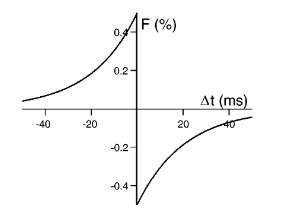
\includegraphics[width=0.7\textwidth]{CN1}
	%\captionof{figure}{Figure 1 of \cite{kingma2017adam}. The change of the peak conductance at a synapse as a function of the timing of pre- and postsynaptic action.}		
\end{minipage}
The parameters $\tau_+, \tau_-$ determine the ranges in which pre- and postsynaptic strengthening and weakening occur. $A_+, A_- >0$ describe the maximum amount of synaptic modification when $\Delta t \rightarrow 0$. The parameters were observed experimentally with $\tau_+ = \tau_- \approx  20 $ ms and $A_+ \approx 0.005$. To ensure that uncorrelated pre- and postsynaptic spikes lead to an overall weakening of the synapses the integral of $F$, i.e. its expectation value, needs to be negative. This requires $A_->A_+$. Thus, the authors set $A_-/A_+ = 1.05$, which is however not unambiguously backed by the data.
We see from the representation of $F$ that presynaptic action potentials preceding postsynaptic spikes lead to an overall strengthening of the synapses whereas presynaptic action potentials following postsynaptic spikes result in a weakening of the synapses. The effects of the adaptation of the synapses increase exponentially the smaller the difference to the postsynaptic spike is. 
\newline \newline 
Given this adaptation function $F$, Song et. al \cite{article} simulate the effects of STDP on excitatory synapses in an integrate-and-fire model neuron with 1000 excitatory and 200 inhibitory synapses.
The inhibitory synapses are kept fixed and receive inputs at a frequency of 10 Hz. The peak conductances of the excitatory synapses are initialised with their maximum values $g_{\max}$. This leads to a very strong excitation of the neuron at the beginning in which the mean input already brings the neuron over its activation threshold. Thus, the spikes don't depend on the excitatory inputs and the synapses are weakened according to the function $F$. This continues until the conductances reach a stationary distribution approaching their limiting values $0$ and $g_{\max}$. In this stationary distribution the excitatory inputs balance the inhibitory effects and the membrane current such that the overall potential is at a level where presynaptic potentials can control the timing of postsynaptic spikes which results in competition between the synapses to maintain this equilibrium.
This observation is underpinned by the following figure \ref{fig:1} since for an input frequency of 10Hz way more excitatory synapses maintain their maximum values $g_{\max}$ compared to an input frequency of 40Hz where most of the synapses are close to zero.
\begin{figure}[H]
	\centering	
	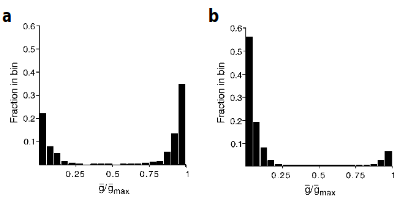
\includegraphics[width=0.7\textwidth]{CN2}
	\caption{Figure 2 of \cite{article} showing the limiting distribution of synaptic conductances. In the left image the input frequency was 10Hz and in the right image the input frequency was 40 Hz.}
	\label{fig:1}
\end{figure}
Song et. al observed further that STDP has a strong regulatory effect on the postsynaptic firing rates, which increases only by 5Hz while the input frequency is raised from 10Hz to 40Hz as displayed in figure \ref{fig:2}. Finally, for all input frequencies the ratio between inhibitory and excitatory conductances is maintained at roughly the same level. This results in a high degree of firing variability and an irregular firing scheme, where postsynaptic spikes follow presynaptic action potentials. 
\begin{figure}[H]
	\centering
	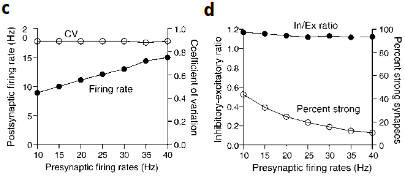
\includegraphics[width=0.7\textwidth]{CN3}
	\caption{Figure 2 of \cite{article} showing the postsynaptic firing rate and the coefficient of variation as a function of the presynaptic firing rates on the left and the In/Ex ratio as well as the percentage of strong synapses on the right.}
	\label{fig:2}
\end{figure}

The proposed method targets two of the main shortcomings of Hebbian synptic plasticity. Firstly, in Hebbian theory synapses are adapted whenever there is correlated pre- and postsynaptic activity. This however, does not have to induce a causal relationship. in STDP synapses are only strengthened if the presynaptic activity preceded the postsynaptic spikes and thus contributed to the activation of the neuron. Secondly, competition arises naturally in STDP in the form of maintaining an equilibrium distribution as opposed to other theories.

However, STDP still requires a few assumptions to reach the equilibrium distribution like a nonlinear spike-generation process or the negativity of the integral of $F$. Most importantly, in STDP postsynaptic firing is the sole cause for strengthening or weakening of the synapses. If the excitatory synapses are not strong enough for the postsynaptic neuron to reach its action potential, there is no way to strengthen these synapses. Therefore, STDP can only be a part of the puzzle of human learning. 